\chapter{Ranking Context Networks}

So far, our treatment of context networks had made an assumption: context solely consists of events co-occurring with the photo-capture events, and these events are obtained from data sources. The second part of the assumption is not always true in practice. For example, a person's roommate might be a last minute addition to a road trip, who was neither on the email chain or the facebook event, will be ranked very low by the discovery algorithm. A professor whose students are receiving best paper award but was not part of the author list herself might be present at the award ceremony because the conference is being hosted 50 kilometers from her univeristy. Similarly, people at a concert might run into acquaintances because they share the same musical interests. In these cases, the data sources will provide incomplete contextual information which leads the discovery algorithm to rank some candidates poorly.

In this chapter, we will attempt to address this problem of boosting the performance of the CueNet framework by introducing a technique to rank candidates based on their participation profile in previous context networks, personal interests or information. We will present our intuition through a series of examples, and introduce a technique similar to PageRank, which is used to rank pages on the world wide web. In our case, we will rank people in the \texttt{CandidateSet} given set of context networks. Our main differences will lie in the initialization of the score matrix and the propagation of scores \textit{across} the different context networks.

\section{Intuition}

\begin{figure}[t]
\centering
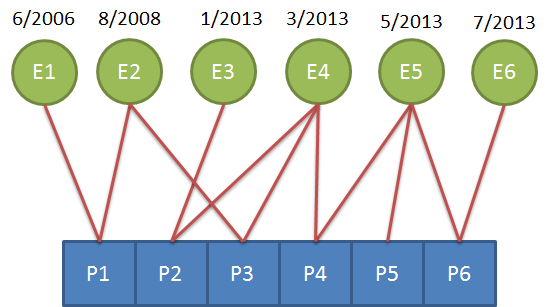
\includegraphics[width=0.65\textwidth]{media/chapter6/intuition-time-example.png}
\caption{Propagating values through temporal relations.}
\label{fig:time-example}
\end{figure}

Consider the very simple context networks shown in figure \ref{fig:time-example}. Each network contains an event, and they have a set of participants. Lets assume that all events \texttt{E1} - \texttt{E6} are of the same type, and occurred at the same location. But as shown in the figure the time of occurrence varies. Lets say that the hit ratio for tagging \texttt{E1} - \texttt{E5} is 100\%. But \texttt{E6} has a few untagged faces, and no more data source is able to provide additional context. The context discovery algorithm has a basic ranking algorithm which looks all social networks (temporal or not), and ranks entities based on whether they have any relations with its participants (in this case, \texttt{P6}). In this case, we could find that \texttt{P6} has participated with \texttt{P5} and \texttt{P4} in event \texttt{E5}. The voting algorithm stops if \texttt{P5} and \texttt{P4} are not found in the \texttt{E6}'s photo. But looking at all the networks, it makes sense to say that since these are all events of the same type, we could say that \texttt{P2}, \texttt{P3} and \texttt{P4} have participated in this same event a few months before \texttt{E6}'s occurrence, and therefore it is possible that \texttt{P2} and \texttt{P3} also participating in \texttt{E6}. With the same idea, we can also \texttt{P2} and \texttt{P1} participated in the same event many years, and therefore is a very low but non-zero chance that \texttt{P1} is present in the photo.

Similarly, look at figure \ref{fig:location-example} where the context networks are exactly as before, but the types of events now vary. We show the type of the event above the event nodes. Their timestamps and location properties are exactly as before. Here, can we exploit some ontological properties about event similarities to propagate scores. If we know that \texttt{L1} is a \texttt{conference}, \texttt{L2} is a \texttt{music-event} and \texttt{L3} is a party, then can we say that \texttt{L2} events are more likely to contain the untagged person than the \texttt{conference} events. 

\begin{figure}[h]
\centering
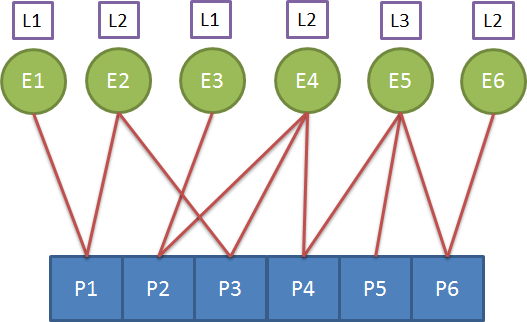
\includegraphics[width=0.65\textwidth]{media/chapter6/intuition-location-example.png}
\caption{Propagating values through ontological event relations.}
\label{fig:location-example}
\end{figure}

Similarly, we can use social and spatial relationships to propagate rank scores to more individuals than just making a single hop as in the context discovery algorithm to reach a wider set of candidates.

\subsection{Rank Propagation}

The rank propagation technique is used to rank nodes in a directed graph. Most commonly seen versions are the HITS algorithm invented by Jon Kleinberg \cite{kleinberg1999authoritative} and the PageRank algorithm developed by Larry Page and Sergey Brin \cite{page1999pagerank}. The idea in the latter is to assign a set of initial values to a subset of nodes, and propagate a fraction of these values to their neighbours. Each iteration of the algorithm propagates their scores to the neighbouring nodes until the overall ordering of the nodes, according to their scores, does not change. In practice, a few iterations ($\leq$ 10) on web scale graphs is sufficient.

In this chapter, we will modify the rank propagation technique to rank entities on a given set of context networks, to determine who might be participating in a new events. We will initialize scores of the nodes on the basis of what is known about the new event -- its type, the participating entities, and propagate the scores based on a set of propagation functions which we will introduce later. Since the basic propagation algorithm is an expensive one, we will look at some ways to reduce the size of the context networks, so the algorithm converges quickly, and still provides useful results.

\section{Preliminaries}

Let us first take a look at how rank propagation works in simple directed graphs. The Pagerank \cite{page1999pagerank} algorithm, designed to rank large web graphs is an extension of this idea. The intuition behind Pagerank is known as the random surfer model. The rank propagation models the behavior of a random web surfer who follows a few links and then gets bored and jumps to a random part of the web graph. The final scores of the ranking algorithm converge to teh probabilities of such a surfer sees a particular page, while traversing the web in this fashion. Consider the graph in figure \ref{fig:pr-graph-example} \footnote{This example is adapted from Wikipedia (http://en.wikipedia.org/wiki/PageRank)}. Let the initial scores of all nodes be 0.25. In the first iteration of the algorithm, the score of node A would be computed as follows. Since A has three incoming edges from nodes B, C and D, each of these nodes would transfer a portion of their score to A. Since B has two outgoing edges, it transfers half of it scores through each of them, C transfers all of its score to A and D transfers one-third of its score to A. At the completion of this iteration, page A has a score of $PR(B)/2 + PR(C) + PR(D)/3 = 0.458$. In this fashion, the scores for all the nodes are computed in each iteration, until the scores converge.

\begin{figure}[t]
\centering
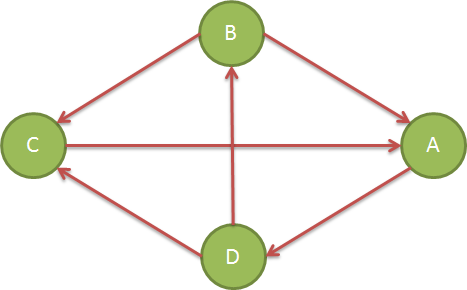
\includegraphics[width=0.65\textwidth]{media/chapter6/pr-example-graph.png}
\caption{Example graph to demonstrate the original Pagerank algorithm.}
\label{fig:pr-graph-example}
\end{figure}

The model introduced by Page and Brin also included a damping factor. Extending the random surfer analogy, this damping factor corresponds to the probability that the surfer stops clicks. At every page the surfer visits, there is a non-zero probability that he will stop surfing. Taking this consideration, the above equation to compute the new pagerank of node A becomes $d(PR(B)/2 + PR(C) + PR(D)/3) = 0.41225$, for d = 0.85. 


\restylealgo{ruled}
\SetAlgoSkip{}
\begin{algorithm}[h!]
\dontprintsemicolon 
\Begin{
  
$R_0$ $\leftarrow$ S  \\
\textbf{loop}: \\
\Indp
  $R_{i+1}$ $\leftarrow$ $AR_i$ \\
  d $\leftarrow$ $||R_i||_1$ - $||R_{i+1}||_1$ \\  
  $R_{i+1}$ $\leftarrow$ $||R_i||_1$ + dE \\
  $\delta$ $\leftarrow$ $||R_{i+1} - R_i||_1$ \\
\Indm
\textbf{while $\delta$ $>$ $\epsilon$}
}
\caption{Original Pagerank Algorithm}
\label{alg:pr-alg}
\end{algorithm}

Mathematically, the pagerank algorithm is expressed as shown in algorithm \ref{alg:pr-alg}. R is a vector over all the nodes in the graph. A is an adjacency matrix where each cell measures is the reciprocal of outgoing edge count. If $u$ and $v$ are two nodes, and there are $N_u$ outgoing edges from $u$ and one of them ends in $v$, then $A(u, v) = 1/N_u$. The expression $||R||_1$ is the L1 or Manhattan norm of a vector $R$, which is computed as $\sum_{\forall i} |R_i|$. The vector $S$ is the initial score assigned to the nodes. On a large scale, pagerank scores are computed using the MapReduce framework \cite{dean2008mapreduce}.

\section{Rank Propagation in Context Networks}

main reason to do this: ranking heterogenous content across different axis.

what are you doing: computing similar kinds of event occurrences on the basis or time, space, type and entity similarities.

\subsection{Propagation Functions}

\begin{itemize}
\item \textbf{Temporal Propagation}:
\item \textbf{Spatial Propagation}:
\item \textbf{Type Propagation}:
\item \textbf{Object Propagation}:
\item \textbf{Structural Propagation}:
\end{itemize}

\section{Experiments}